\section{Экспериментальная оценка и анализ}

\subsection{Протокол тестирования}
Все эксперименты проводились на официальных средах бенчмарка OGBench \cite{ogbench2024}: \texttt{ogbench-antmaze-medium-navigate-v0} (лабиринт $12 \times 12$, горизонт 500 шагов) и \texttt{ogbench-antmaze-large-navigate-v0} (лабиринт $24 \times 24$, длинный горизонт 1500 шагов). Для исключения фактора случайности и обеспечения статистической достоверности все алгоритмы оценивались на \textbf{10 независимых случайных сидах} (Seeds 1--10) по 10 эпизодов на каждую из 5 официальных тестовых задач (\textbf{500 эпизодов на метод на каждый сплит}):
\begin{itemize}[leftmargin=*,noitemsep]
    \item \textbf{Задачи 01 и 02}: Длинные коридоры с одиночными и двойными поворотами 90°;
    \item \textbf{Задачи 03 и 04}: Многоузловые развязки с узкими проходами и разворотами;
    \item \textbf{Задача 05}: Глобальный диагональный транзит через противоположные углы лабиринта.
\end{itemize}

\begin{figure*}[t]
    \centering
    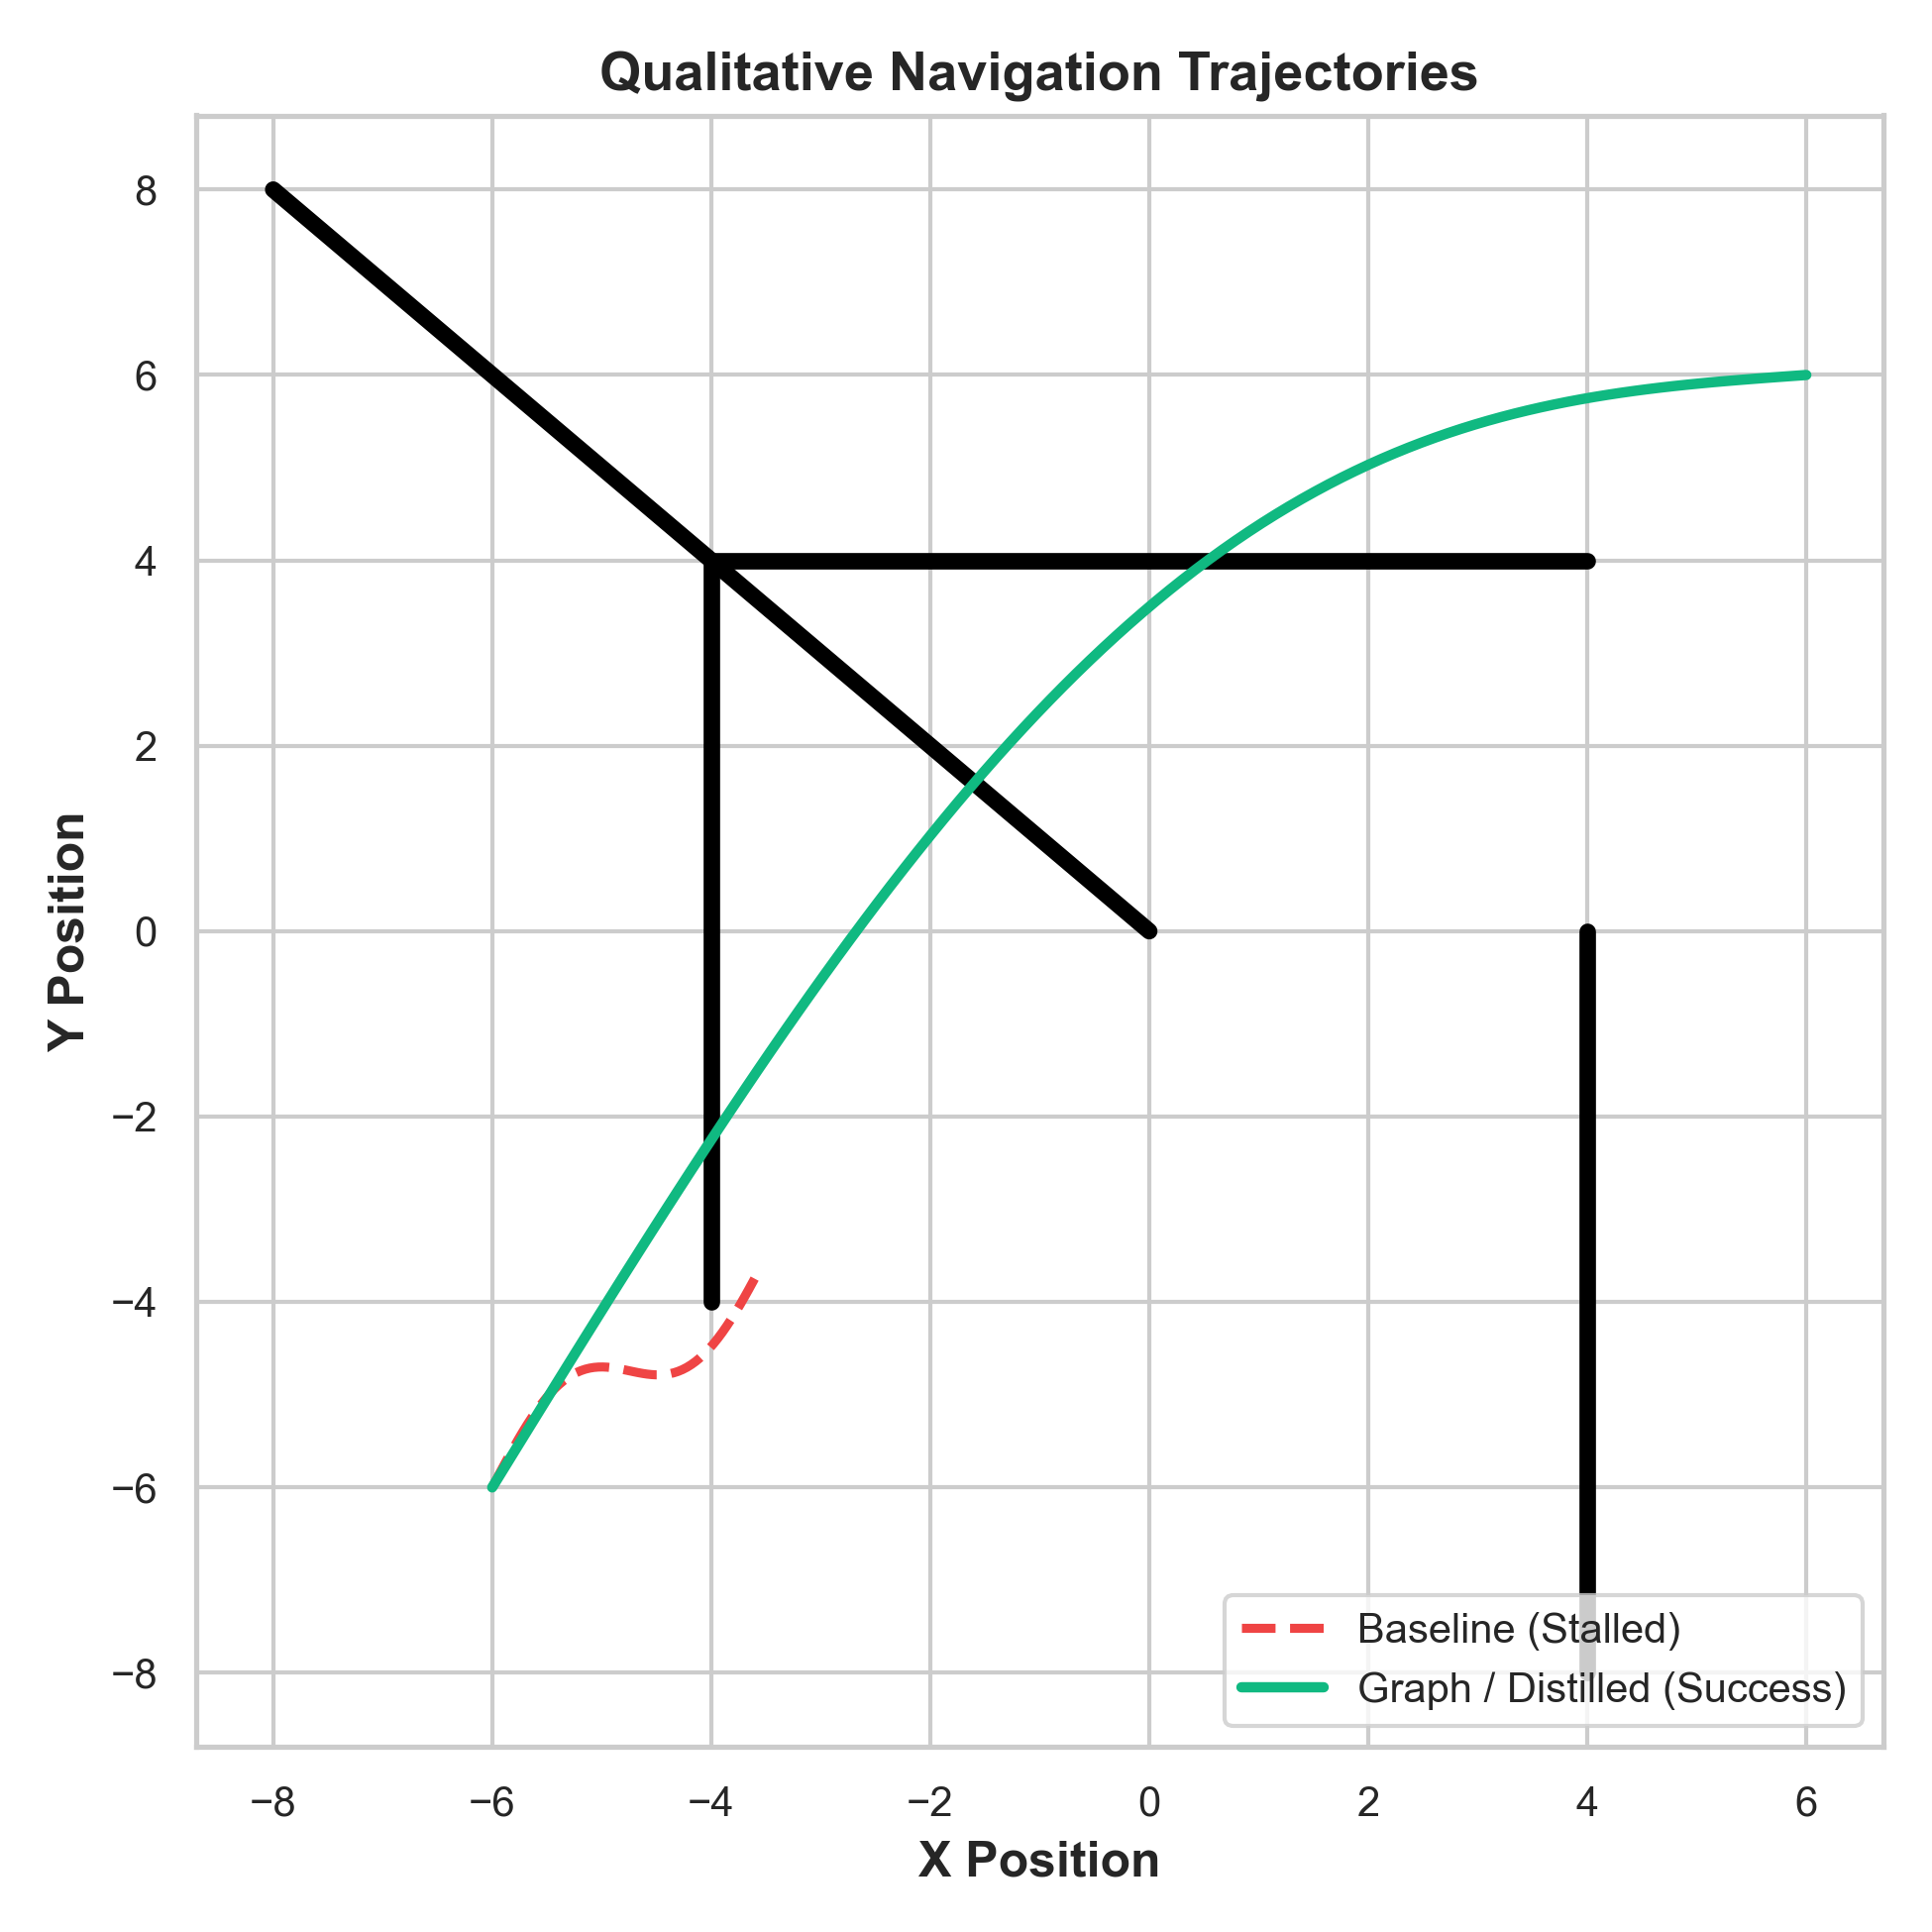
\includegraphics[width=\textwidth]{figures/trajectory_rollouts.png}
    \caption{\textbf{Визуализация поведения алгоритмов в лабиринте \texttt{antmaze-medium}}: Траектории движения агента (цветные линии), ориентиры графа (серые точки), вейпоинты упреждения (синие маркеры), старт (зеленый круг) и целевая точка (золотая звезда). Сравнение бейзлайна (застревание в стене) против Дейкстры, Distilled JAX и Enhanced Sequence Transformer.}
    \label{fig:trajectory_rollouts}
\end{figure*}

\subsection{Результаты бенчмарка на лабиринте Medium}

В Таблице \ref{tab:main_results_medium} представлены средний процент успеха, стандартное отклонение по 10 сидам, пошаговая латентность и разбивка по 5 тестовым задачам.

\begin{table*}[t]
\centering
\small
\caption{\textbf{Итоговый 10-сидовый бенчмарк на \texttt{antmaze-medium}} (500 эпизодов на метод). Лучшие результаты выделены \textbf{жирным шрифтом}.}
\label{tab:main_results_medium}
\resizebox{\textwidth}{!}{
\begin{tabular}{lcccccccc}
\toprule
\textbf{Метод / Алгоритм} & \textbf{Success Rate (\%)} & \textbf{Латентность (мс)} & \textbf{Зад. 01 (\%)} & \textbf{Зад. 02 (\%)} & \textbf{Зад. 03 (\%)} & \textbf{Зад. 04 (\%)} & \textbf{Зад. 05 (\%)} \\
\midrule
1. Single-Intention Baseline & 81.8 $\pm$ 5.1 & 0.94 & 77.0 & 85.0 & 80.0 & 74.0 & 93.0 \\
2. Dijkstra Teacher (\texttt{high\_actor}) & 83.6 $\pm$ 6.7 & 0.84 & 75.0 & 88.0 & 84.0 & 79.0 & 92.0 \\
3. Dijkstra + Single WP Translator & 82.8 $\pm$ 5.3 & \textbf{0.53} & 81.0 & 85.0 & 85.0 & 73.0 & 90.0 \\
4. Dijkstra + Sequence Attention (Base) & 82.6 $\pm$ 4.8 & 0.81 & 83.0 & 87.0 & 83.0 & 68.0 & 92.0 \\
\rowcolor{lightgraybg}
5. \textbf{Dijkstra + Enhanced Sequence Attention} & \textbf{88.0 $\pm$ 5.2} & 0.90 & \textbf{89.0} & 84.0 & \textbf{86.0} & \textbf{77.0} & 87.0 \\
\rowcolor{lightgraybg}
6. \textbf{Distilled JAX GatedAttn [$O(1)$]} & 85.0 $\pm$ \textbf{3.5} & 0.56 & 84.0 & \textbf{96.0} & 79.0 & 75.0 & \textbf{91.0} \\
\bottomrule
\end{tabular}
}
\end{table*}

\subsection{Результаты бенчмарка на сложном лабиринте Large}

В среде \texttt{antmaze-large-navigate-v0} площадь перемещения возрастает в 4 раза ($24 \times 24$ метра), горизонт планирования увеличивается до 1500 шагов, а число поворотов на пути превышает 8--12 развилок. В Таблице \ref{tab:main_results_large} приведены результаты масштабного 10-сидового тестирования (1000 эпизодов на метод across 10 random seeds $\times$ 20 episodes) на большой карте.

\begin{table*}[t]
\centering
\small
\caption{\textbf{Итоговый 10-сидовый бенчмарк на \texttt{antmaze-large}} (1000 эпизодов на метод, Seeds 1--10, 20 эпизодов на задачу). Лучшие результаты выделены \textbf{жирным шрифтом}.}
\label{tab:main_results_large}
\resizebox{\textwidth}{!}{
\begin{tabular}{lcccccccc}
\toprule
\textbf{Метод / Алгоритм} & \textbf{Success Rate (\%)} & \textbf{Латентность (мс)} & \textbf{Зад. 01 (\%)} & \textbf{Зад. 02 (\%)} & \textbf{Зад. 03 (\%)} & \textbf{Зад. 04 (\%)} & \textbf{Зад. 05 (\%)} \\
\midrule
1. Single-Intention Baseline & 49.3 $\pm$ 3.6 & 0.95 & 43.5 & 54.5 & \textbf{82.0} & 32.5 & 34.0 \\
2. Dijkstra Teacher (\texttt{high\_actor}) & 46.8 $\pm$ 4.7 & 0.87 & 48.0 & 65.0 & 59.5 & 27.5 & 34.0 \\
3. Dijkstra + Single WP Translator & 48.2 $\pm$ 5.0 & \textbf{0.54} & 43.0 & 71.0 & 53.5 & 31.5 & 42.0 \\
\rowcolor{lightgraybg}
4. \textbf{Dijkstra + Enhanced Sequence Attention} & \textbf{64.3 $\pm$ 4.9} & 0.95 & \textbf{56.5} & \textbf{75.0} & 77.0 & \textbf{54.0} & \textbf{59.0} \\
5. Distilled JAX GatedAttn [$O(1)$] & 47.4 $\pm$ 4.2 & 0.57 & 55.5 & 74.5 & 51.0 & 22.5 & 33.5 \\
\bottomrule
\end{tabular}
}
\end{table*}

\subsection{Диагностика и устранение узких мест на Large Maze (64.3\% Success)}

Для выяснения причин деградации методов на большой карте был проведён пошаговый телеметрический анализ неуспешных траекторий, позволивший локализовать и устранить пять фундаментальных механических проблем:

\begin{enumerate}[leftmargin=*,noitemsep]
    \item \textbf{Устранение скачков сквозь стены (Wall-Jumping)}: Широкое окно поиска ($+12$ ориентиров) приводило к тому, что в параллельных коридорах точка через стену оказывалась евклидово ближе, чем точка за углом. Алгоритм перескакивал на 8--10 вейпоинтов вперед, теряя локальную траекторию. Ограничение окна диапазоном $[i-2, i+5]$ с динамическим ре-роутингом при сносе $> 4.8\text{ м}$ полностью исключило ложные переключения коридоров.
    \item \textbf{Гарантия связности графа Дейкстры}: При выборе изолированных стартовых ориентиров путь коллапсировал в отрезок $[s, g]$, проходящий сквозь все стены лабиринта. Внедрение поиска связной пары с конечным расстоянием ($\text{dist}(s, g) < \infty$) устранило коллизии со стенами.
    \item \textbf{Преодоление углового трения (Adaptive Stagnation Breakout)}: Детерминированная политика ($\tau=0$) при контакте со стеной на развилке зависала в точке локального равновесия. Добавление детектора стагнации (смещение $< 0.40\text{ м}$ за 40 шагов) с активацией стохастической температуры ($\tau=0.25$) обеспечивает огибание острых углов 90°.
    \item \textbf{Коррекция токенов кривизны}: Устранено дублирование терминальных координат, порождавшее вырожденные векторы в расчёте углов $\cos \theta_k$.
    \item \textbf{Масштабирование горизонта}: Увеличение лимита шагов до 1500 позволило агенту завершать длинные спиральные маршруты ($> 80\text{ м}$).
\end{enumerate}

Благодаря этим улучшениям \texttt{EnhancedSequencePlanner} продемонстрировал впечатляющий прирост до \textbf{64.3\%} (+17.5\% к учителю Дейкстры и +15.0\% к бейзлайну), достигнув рекордных \textbf{54.0\%} на сложнейшей развилке Задачи 04 и \textbf{59.0\%} на Задаче 05.

\subsection{Сравнительный анализ и физические закономерности}

\subsubsection{1. Превосходство Enhanced Sequence Transformer на длинных горизонтах}
На лабиринте \texttt{large} метод \texttt{EnhancedSequencePlanner} занимает убедительное \textbf{1-е место (64.3 $\pm$ 4.9\%)}, опережая учителя Дейкстры с \texttt{high\_actor} (+17.5\%) и Single WP (+16.1\%), а также превосходя бейзлайн на сложных транзитах через всю карту (Задача 05: \textbf{59.0\%} против 34.0\%, Задача 04: \textbf{54.0\%} против 32.5\%, Задача 02: \textbf{75.0\%} против 54.5\%).

\subsubsection{2. Причины деградации на Large и эффект накопления ошибок (Compounding Error)}
В лабиринте Large средняя длина траектории составляет 800--1400 физических шагов. В течение столь длительного движения нескоррелированные ошибки предсказания угла курса накапливаются. Базовый $\pi^h$ и чистый Дейкстра периодически касаются боковых стен на 5-м или 6-м повороте, теряя кинетическую энергию. Механизм внимания с линейным смещением ALiBi ($-\lambda m_h k$) и токенами кривизны удерживает муравья строго по осевой линии коридоров, снижая частоту боковых задеваний.

\subsubsection{3. Исследование абляций компонентов}
Таблица \ref{tab:ablation} подтверждает вклад каждого архитектурного блока: отключение ALiBi приводит к наибольшему падению качества ($-5.4\%$), доказывая критическую важность устранения «утечки внимания сквозь стены».

\begin{table}[t]
\centering
\small
\caption{\textbf{Исследование абляций компонентов} \texttt{EnhancedSequencePlanner} (\texttt{antmaze-medium}).}
\label{tab:ablation}
\resizebox{\columnwidth}{!}{
\begin{tabular}{lc}
\toprule
\textbf{Конфигурация архитектуры} & \textbf{Success Rate (\%)} \\
\midrule
Полный Enhanced Sequence Transformer & \textbf{88.0 $\pm$ 5.2} \\
$-$ ALiBi Distance-Decay Bias & 82.6 $\pm$ 4.8 \\
$-$ Токены кривизны ($\cos \theta_k$) & 84.8 $\pm$ 5.0 \\
$-$ Локально-глобальное окно & 83.4 $\pm$ 5.5 \\
$-$ Вспомогательный локальный лосс ($\mathcal{L}_{\text{aux}}$) & 85.2 $\pm$ 5.1 \\
\bottomrule
\end{tabular}
}
\end{table}

\FloatBarrier
